
\newpage
\section{Capturing and Analyzing FTP Traffic}

\subsection{Activity}

\noindent {\bf{Bước 1:}} Khởi động máy ảo Windows 10 và bật ứng dụng Wireshark. Chọn \textbf{Ethernet} để lấy thông tin chuyển tải. Sau đó chọn \textbf{Start} để bắt đầu hoặc Stop để dừng lại.

\begin{figure}[!htb]
    \centering
    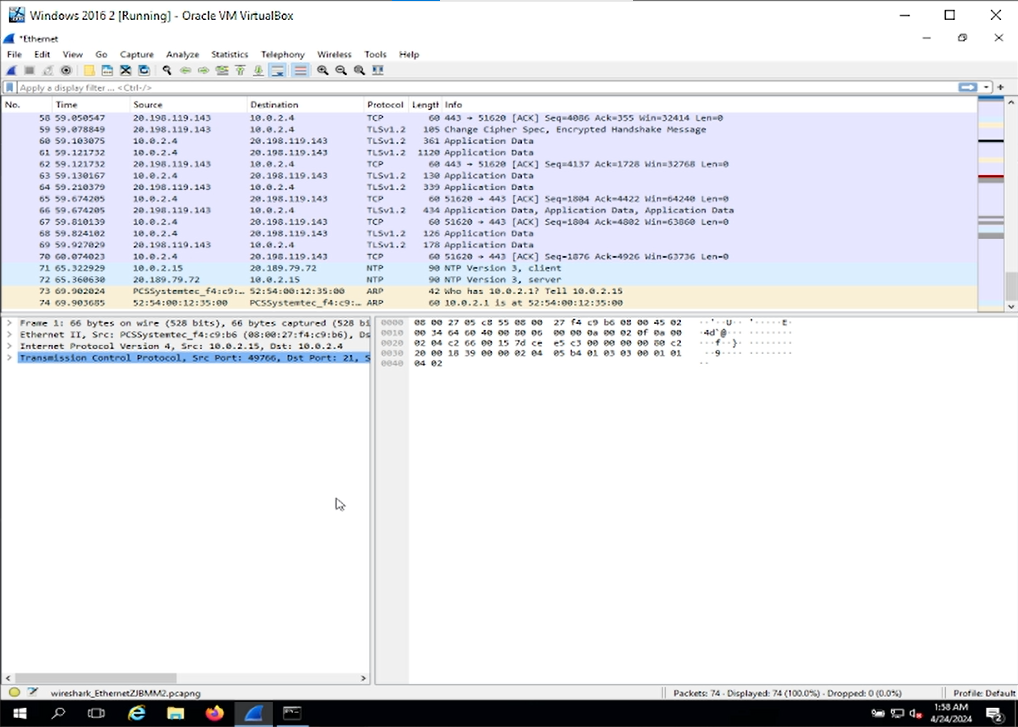
\includegraphics[width=0.75\linewidth]{figure//chapter9//lab9_3/wireshark.png}
    \caption{Khởi động Wireshark}
    \label{fig:enter-label}
\end{figure}



\noindent {\bf{Bước 2:}} Bật \textbf{cmd} rồi nhập lệnh \textbf{cd /}. Sau đó, nhập \textbf{ftp WindowsServer\_IP}.

\begin{figure}[!htb]
    \centering
    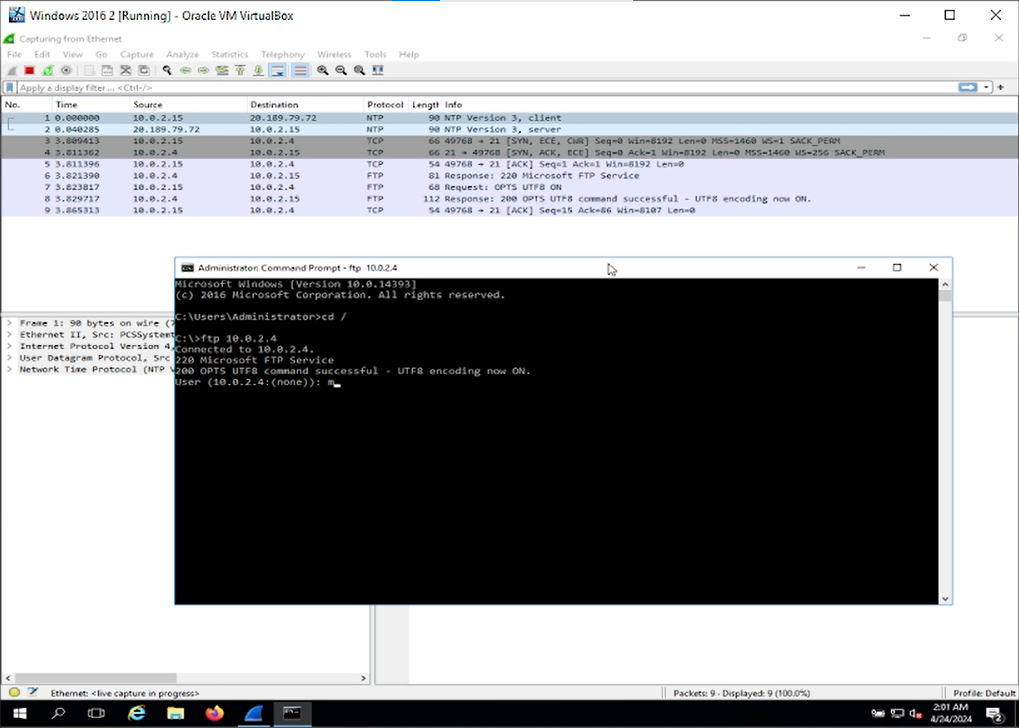
\includegraphics[width=0.75\linewidth]{figure//chapter9//lab9_3/login_ftp.png}
    \caption{Đăng nhập vào FTP Server}
    \label{fig:enter-label}
\end{figure}

\newpage

\noindent {\bf{Bước 3:}} Đăng nhập với tên là \textbf{mbloom}. Nếu chưa có tài khoản thì có thể tự tạo mới ở \textbf{Active Directory Users and Computers}. Mật khẩu là \textbf{Pa\$\$word}. Chạy lệnh \textbf{dir} sẽ thấy có file \textbf{Credentials.txt} được tạo ở phần 2.

\begin{figure}[!htb]
    \centering
    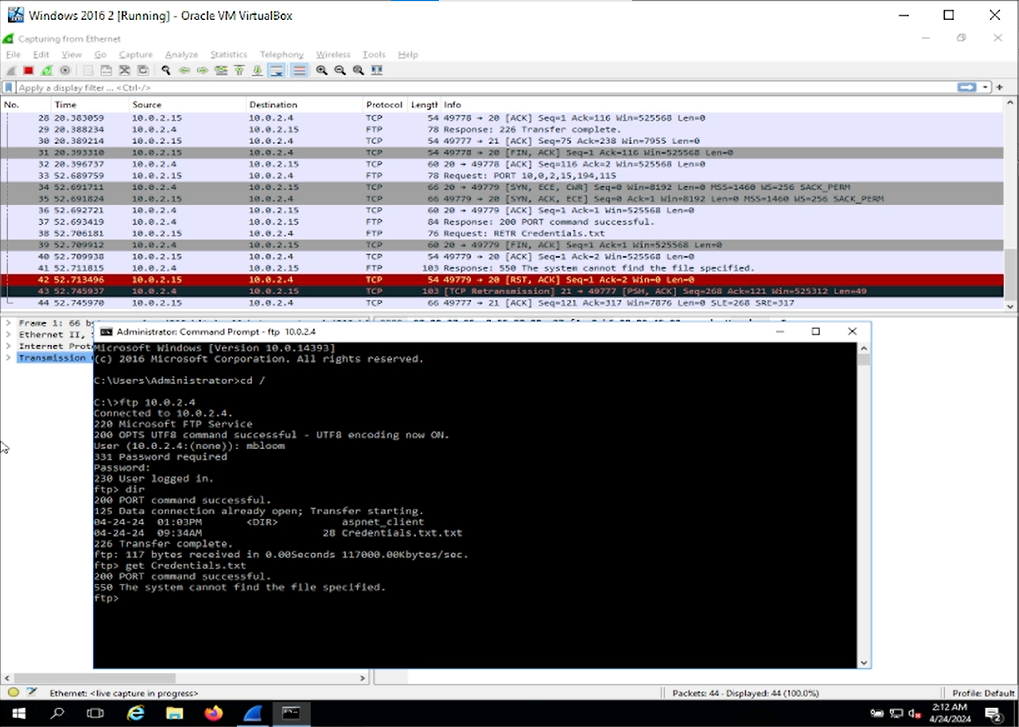
\includegraphics[width=1\linewidth]{figure//chapter9//lab9_3/login_ftp_server.png}
    \caption{Đăng nhập với mbloom và chạy lệnh dir}
    \label{fig:enter-label}
\end{figure}

\noindent {\bf{Bước 4:}} Tải tệp \textbf{Credentials.txt} bằng lệnh \textbf{get Credentials.txt}. Sau đó, nhập lệnh \textbf{bye} để thoát \textbf{FTP Server}.

\begin{figure}[!htb]
    \centering
    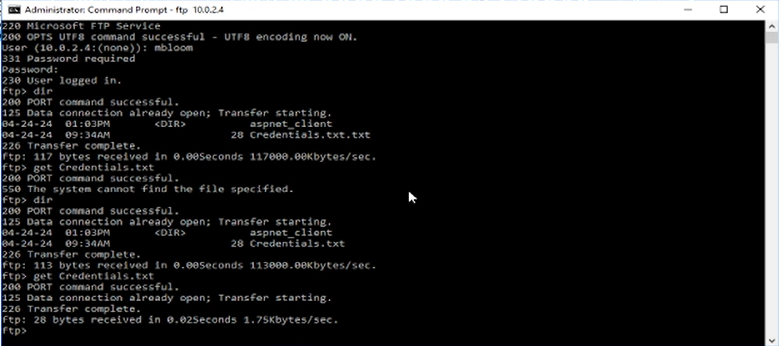
\includegraphics[width=1\linewidth]{figure//chapter9//lab9_3/get_file.png}
    \caption{Tải file Credentials.txt}
    \label{fig:enter-label}
\end{figure}

\newpage

\noindent {\bf{Bước 5:}} Quay lại Wireshark và khám phá output. Bạn có thể thấy có nhiều địa chỉ IP không thuộc vào máy Windows 10 và FTP Server. Khi đó, chọn \textbf{Capture} và \textbf{Capture Filters} để lọc message. 

\begin{figure}[!htb]
    \centering
    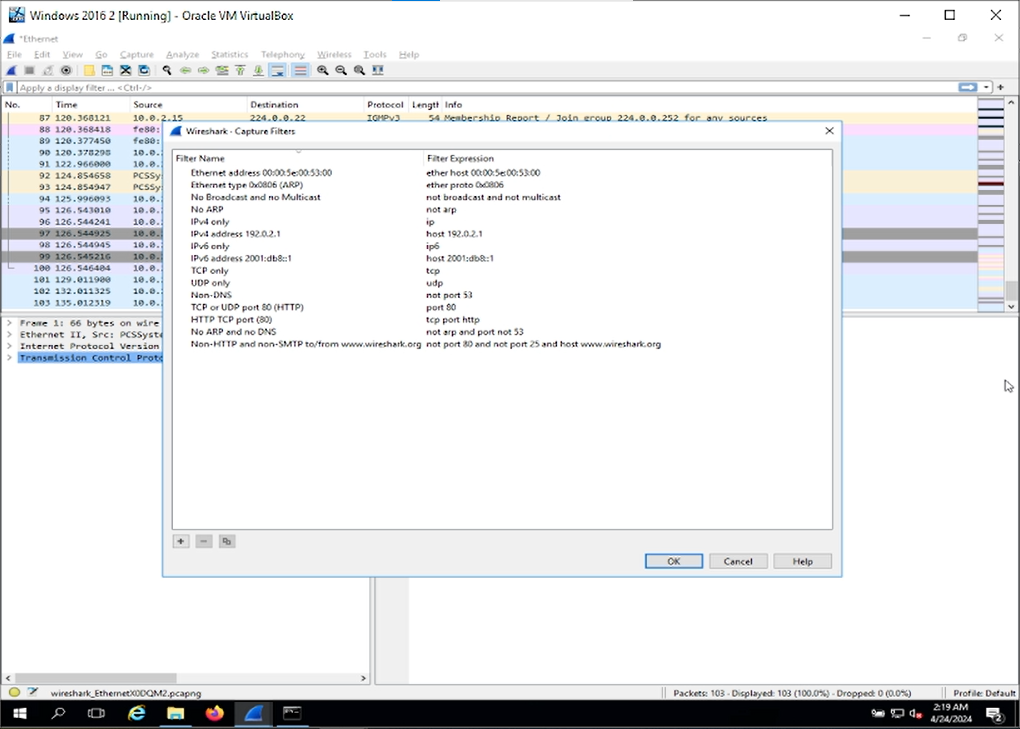
\includegraphics[width=0.9\linewidth]{figure//chapter9//lab9_3/capture-filters.png}
    \caption{Màn hình Capture Filters}
    \label{fig:enter-label}
\end{figure}

\noindent Lúc này các message được lọc sẽ có các địa chỉ IP của Windows 10 và FTP Server.

Cuối cùng quay trở lại và bật tường lửa lên như cũ và tắt máy.

\subsection{Review Questions}

\noindent Câu 1:

A: Require users to authenticate using their domain account.

\noindent Câu 2: 

A: FTP Data.

\noindent Câu 3: 

C: Windows 10 VM initiated the connection by sending to the FTP server a packet with TCP flag SYN set.

\noindent Câu 4: 

D: The FTP server was not first contacted by Windows VM, it advertised its FTP server, and Windows 10 VM responded.

\noindent Câu 5:

D: The teardown of the TCP session began when Windows 10 VM sent a packet to the FTP server with the TCP flags FIN and ACK set.